% --- Generative simulators vs.\ JEPA ---
\begin{frame}{Generative Simulators: Video Generation as a World Model}
  \begin{itemize}\itemsep0.28em
    \item Large video generators are increasingly pitched as world simulators; most build on diffusion or autoregressive generation (covered earlier in the course).
    \item \textbf{Sora} (OpenAI, 2024) frames video generation explicitly as ``world simulation''; \textbf{GAIA-1} and its successors (Wayve) generate driving scenarios for autonomous-vehicle development.
    \item \textbf{Genie} (Google DeepMind) makes \textbf{playable} worlds: the model predicts the next frames \emph{given user actions}, which is exactly the world-model interface, realized in pixel space. Genie 3 (2025) is reported to run interactive worlds in real time at 720p.
    \item The debate: photorealistic video is not the same as physically consistent prediction. Failures in object permanence and physics are common, and evaluating a simulator's ``correctness'' is an open problem.
  \end{itemize}
\end{frame}

\begin{frame}[t]{Generative world models}
  \centering
  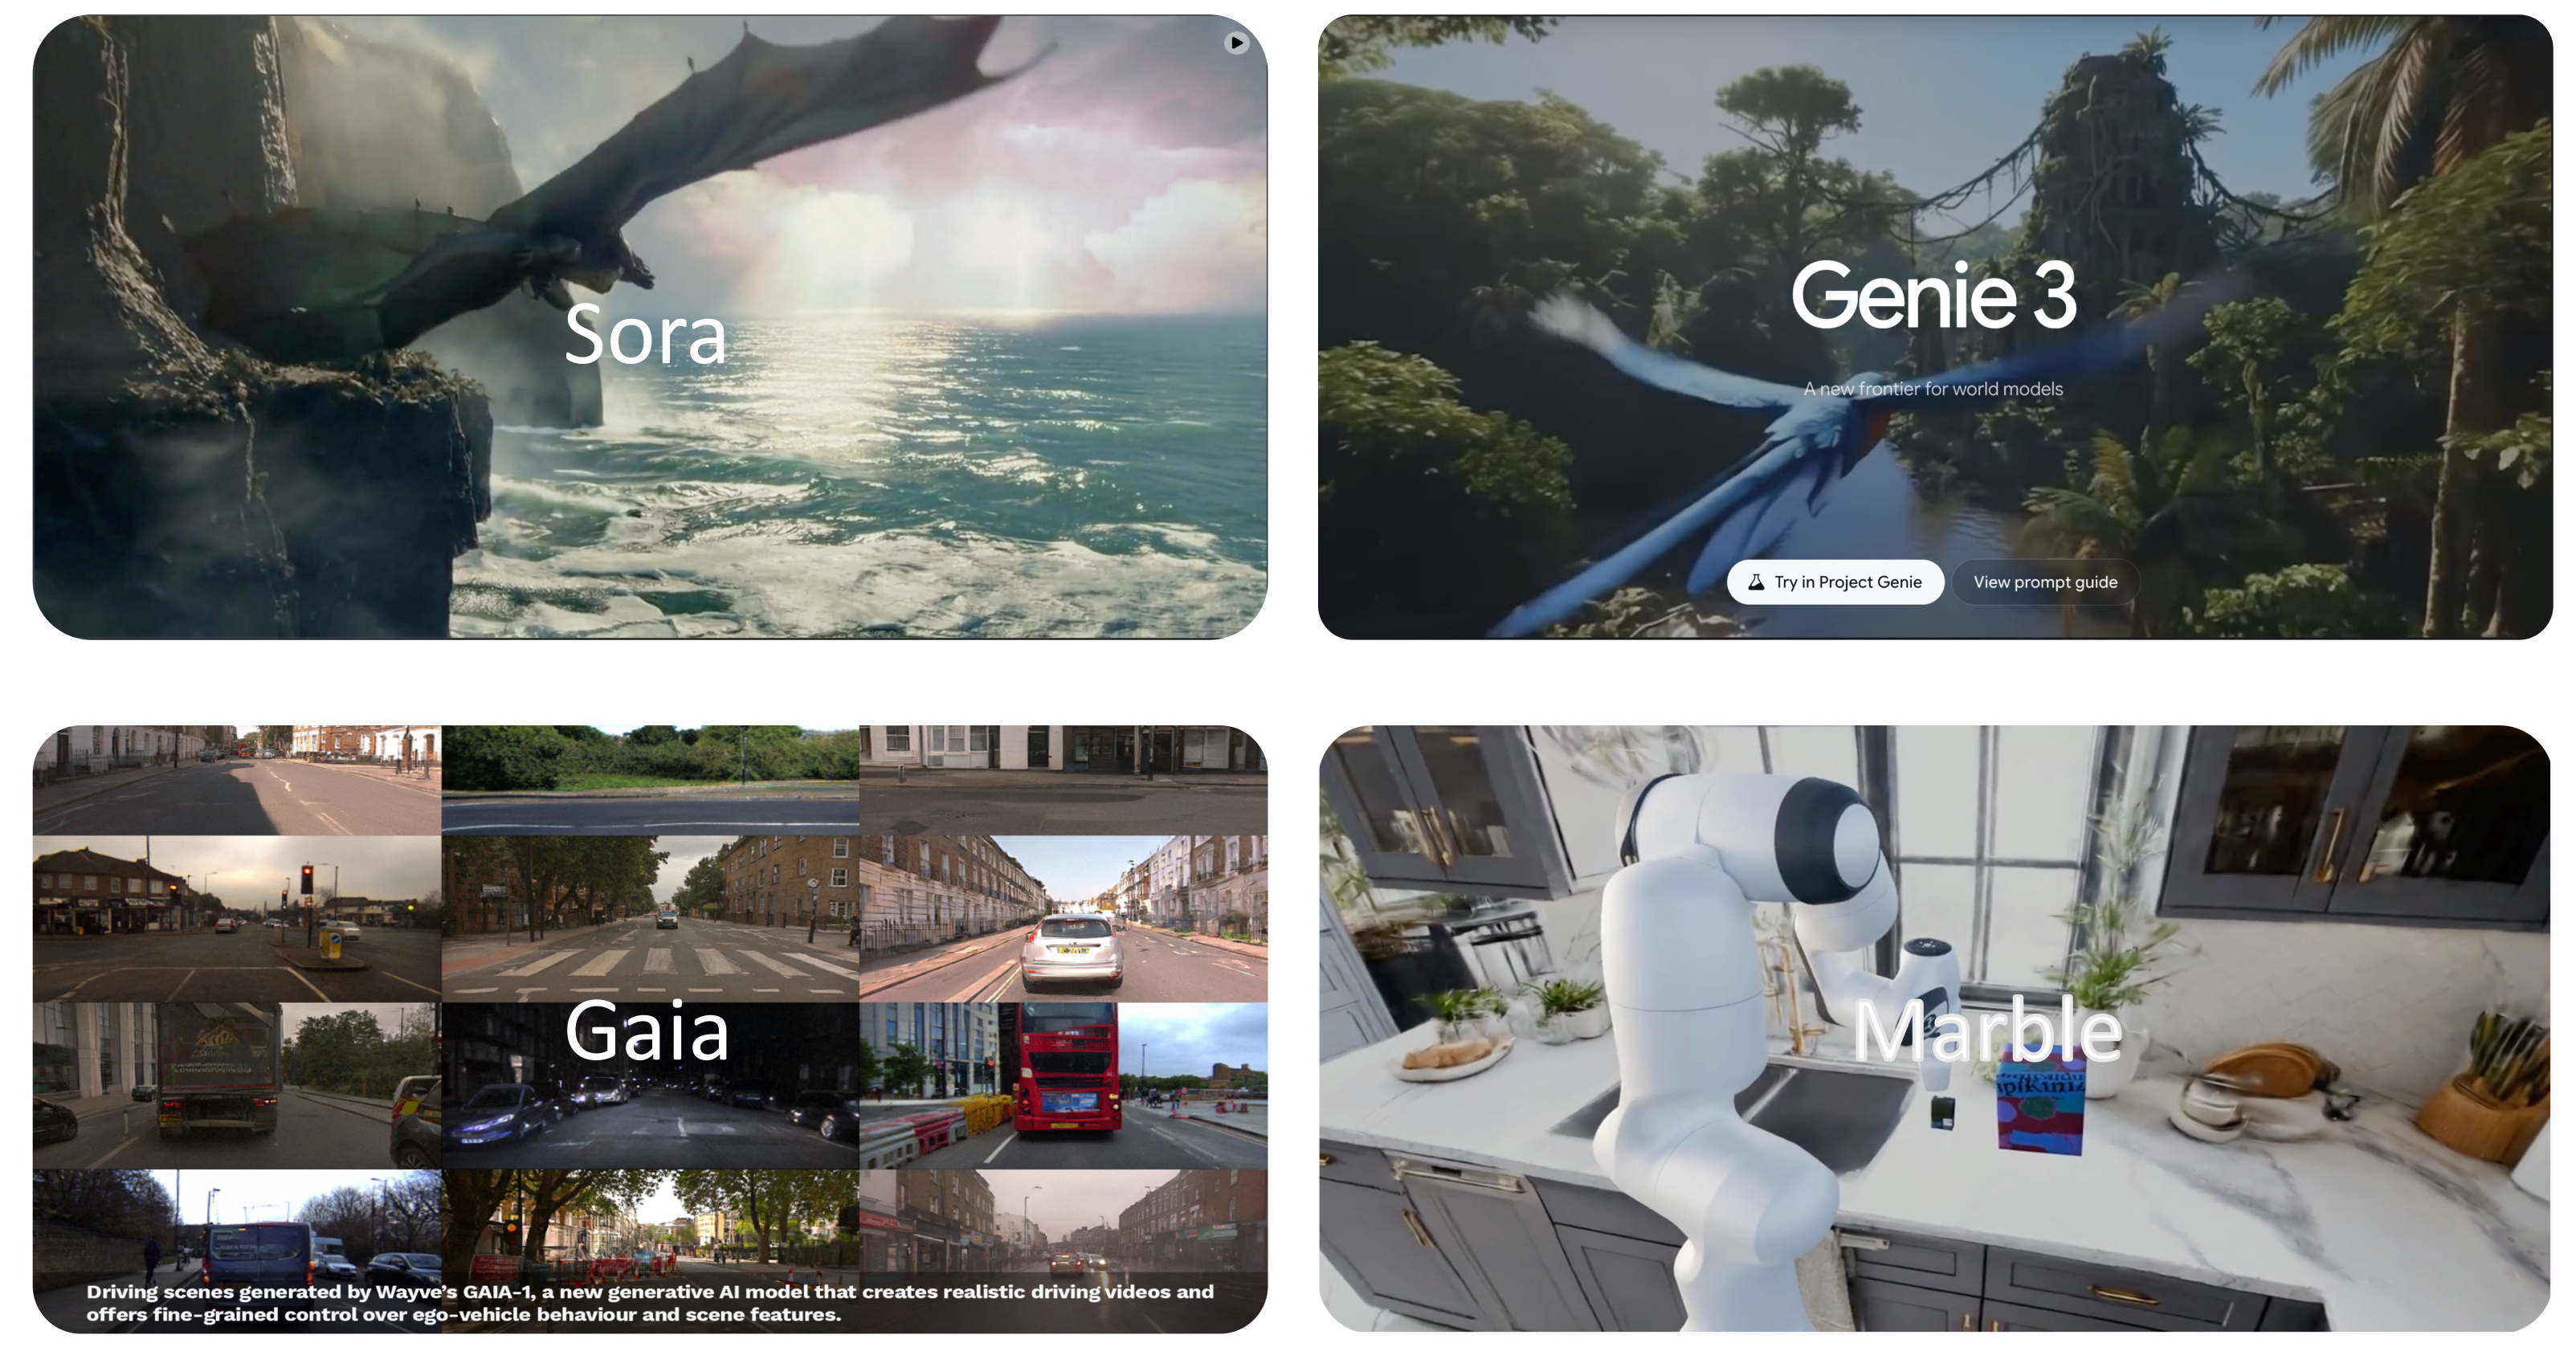
\includegraphics[width=0.76\linewidth,height=0.76\textheight,keepaspectratio]{images/world-models/jepa_cs25_sl04_generative_world_models_sora_gaia.png}\\[0.04em]
  {\scriptsize Image credit: \href{https://drive.google.com/file/d/1bF5Yfzf-FG5iNIAgsXn2DwVD3l3ymvZW/view}{CS25}.}
\end{frame}

\begin{frame}[t]{Architectures: Generative vs.\ Joint Embedding}
  \centering
  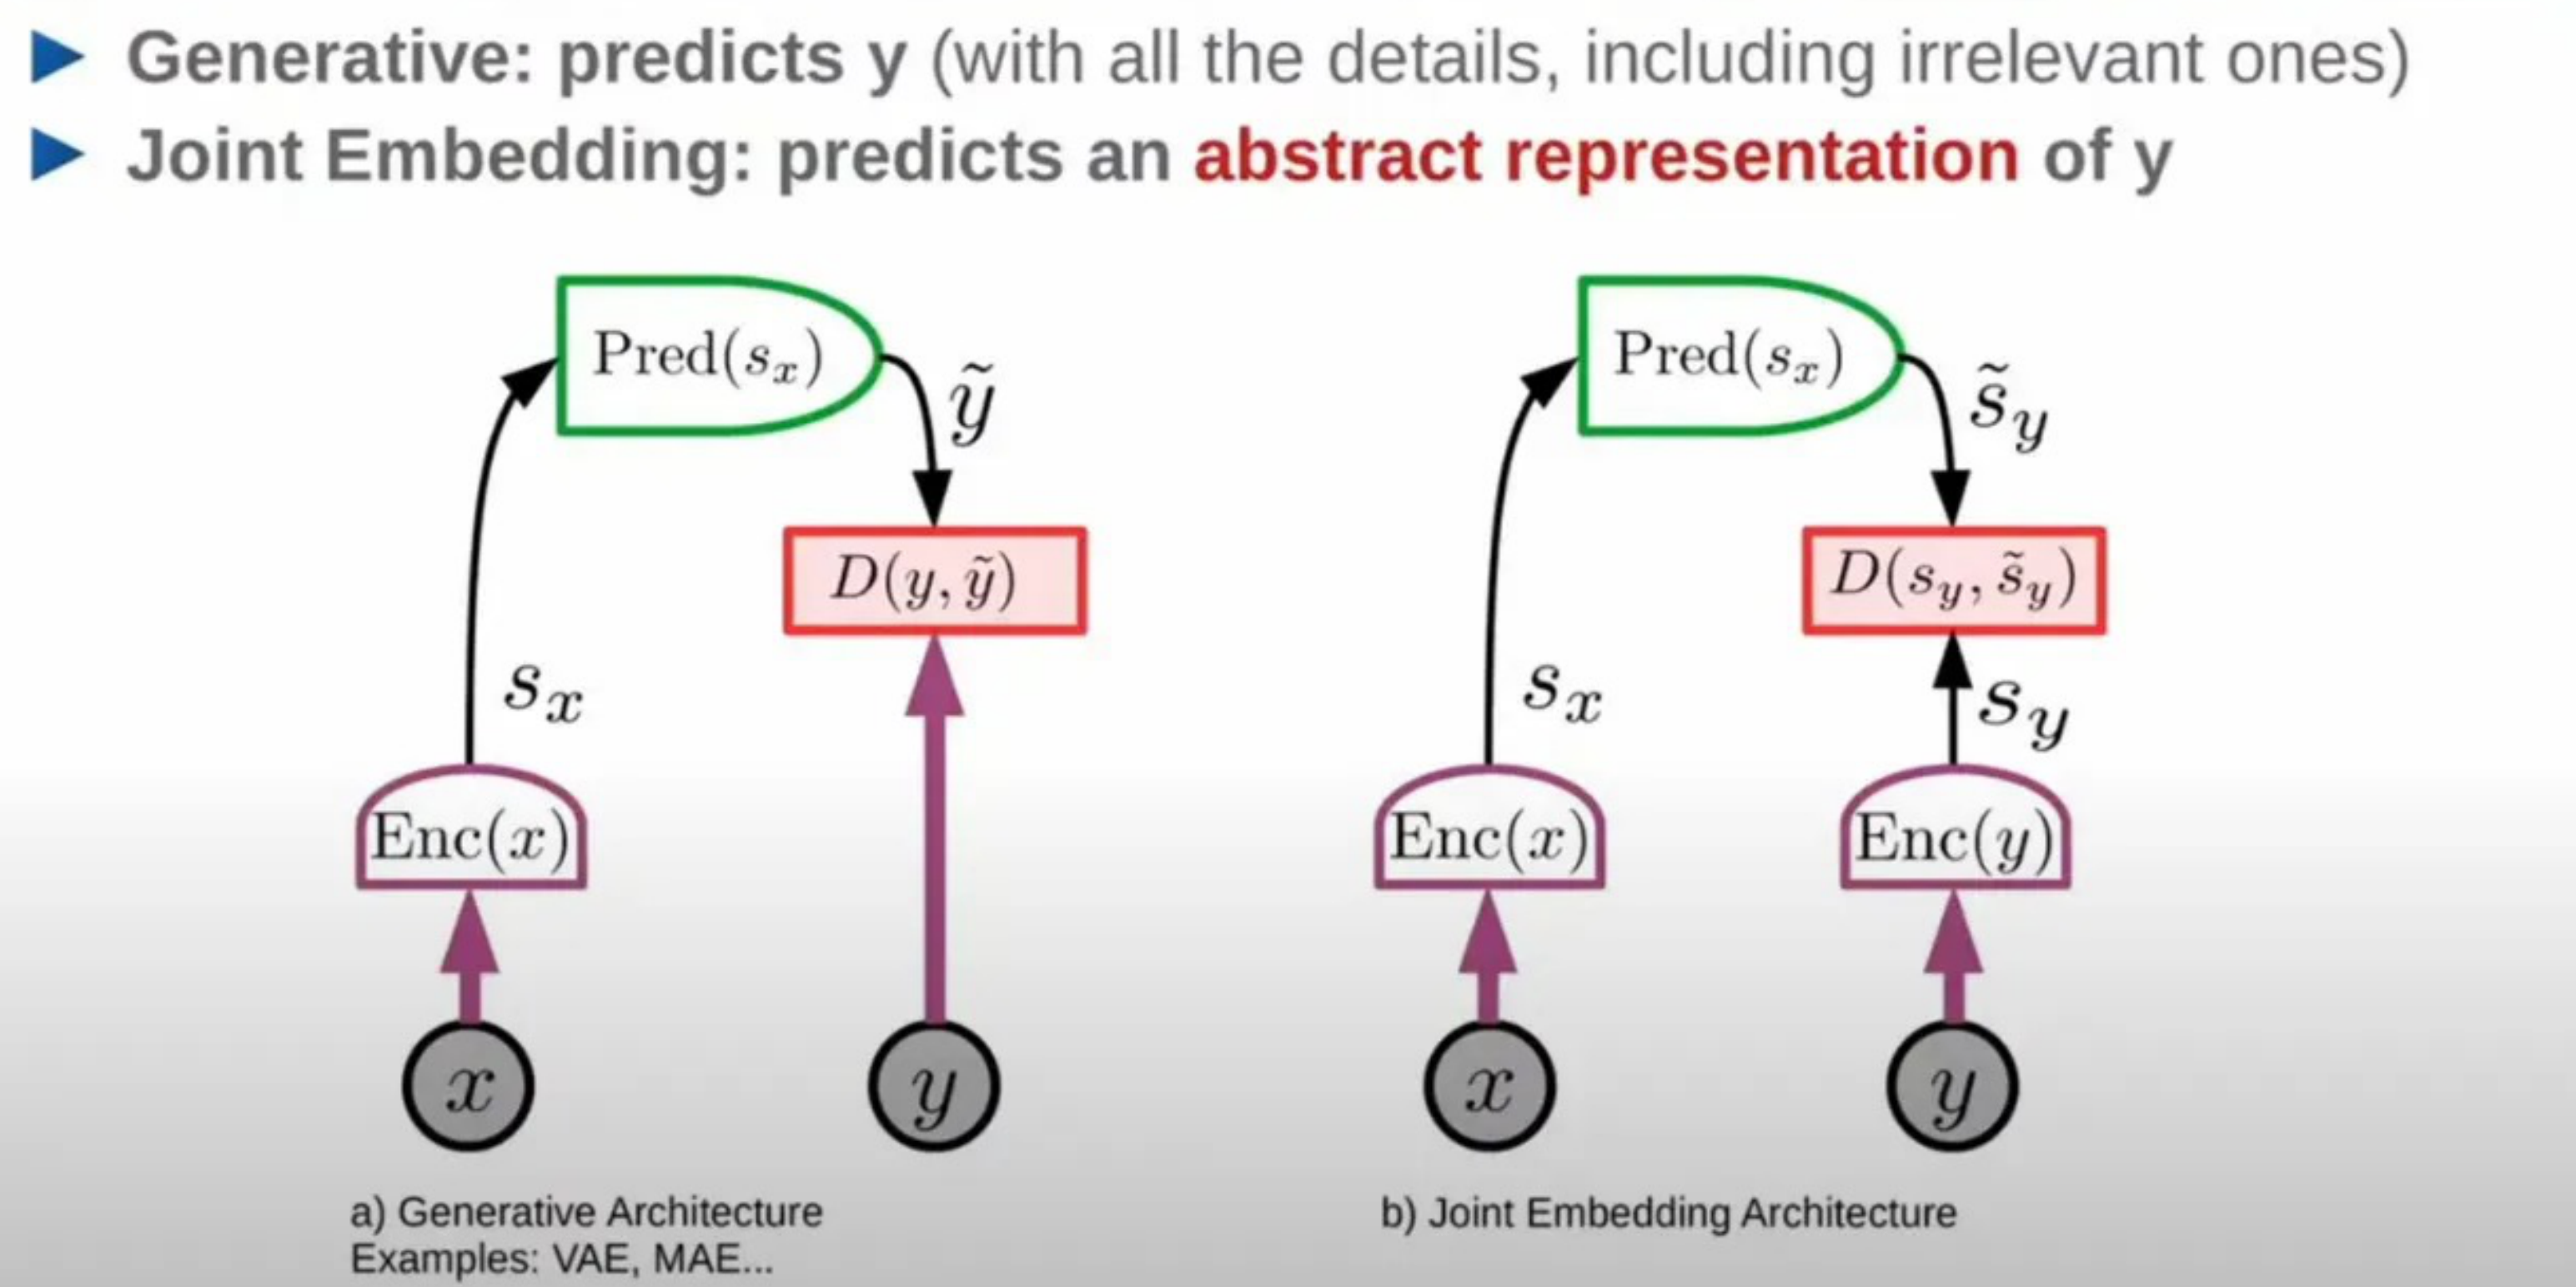
\includegraphics[width=\linewidth,height=0.82\textheight,keepaspectratio]{images/world-models/jepa_cs25_sl05_lecun_world_model_figure.png}\\[0.08em]
  {\scriptsize Image credit: \href{https://drive.google.com/file/d/1bF5Yfzf-FG5iNIAgsXn2DwVD3l3ymvZW/view}{CS25}.}
\end{frame}

\begin{frame}[t]{JEPA \& energy-based view}
  \centering
  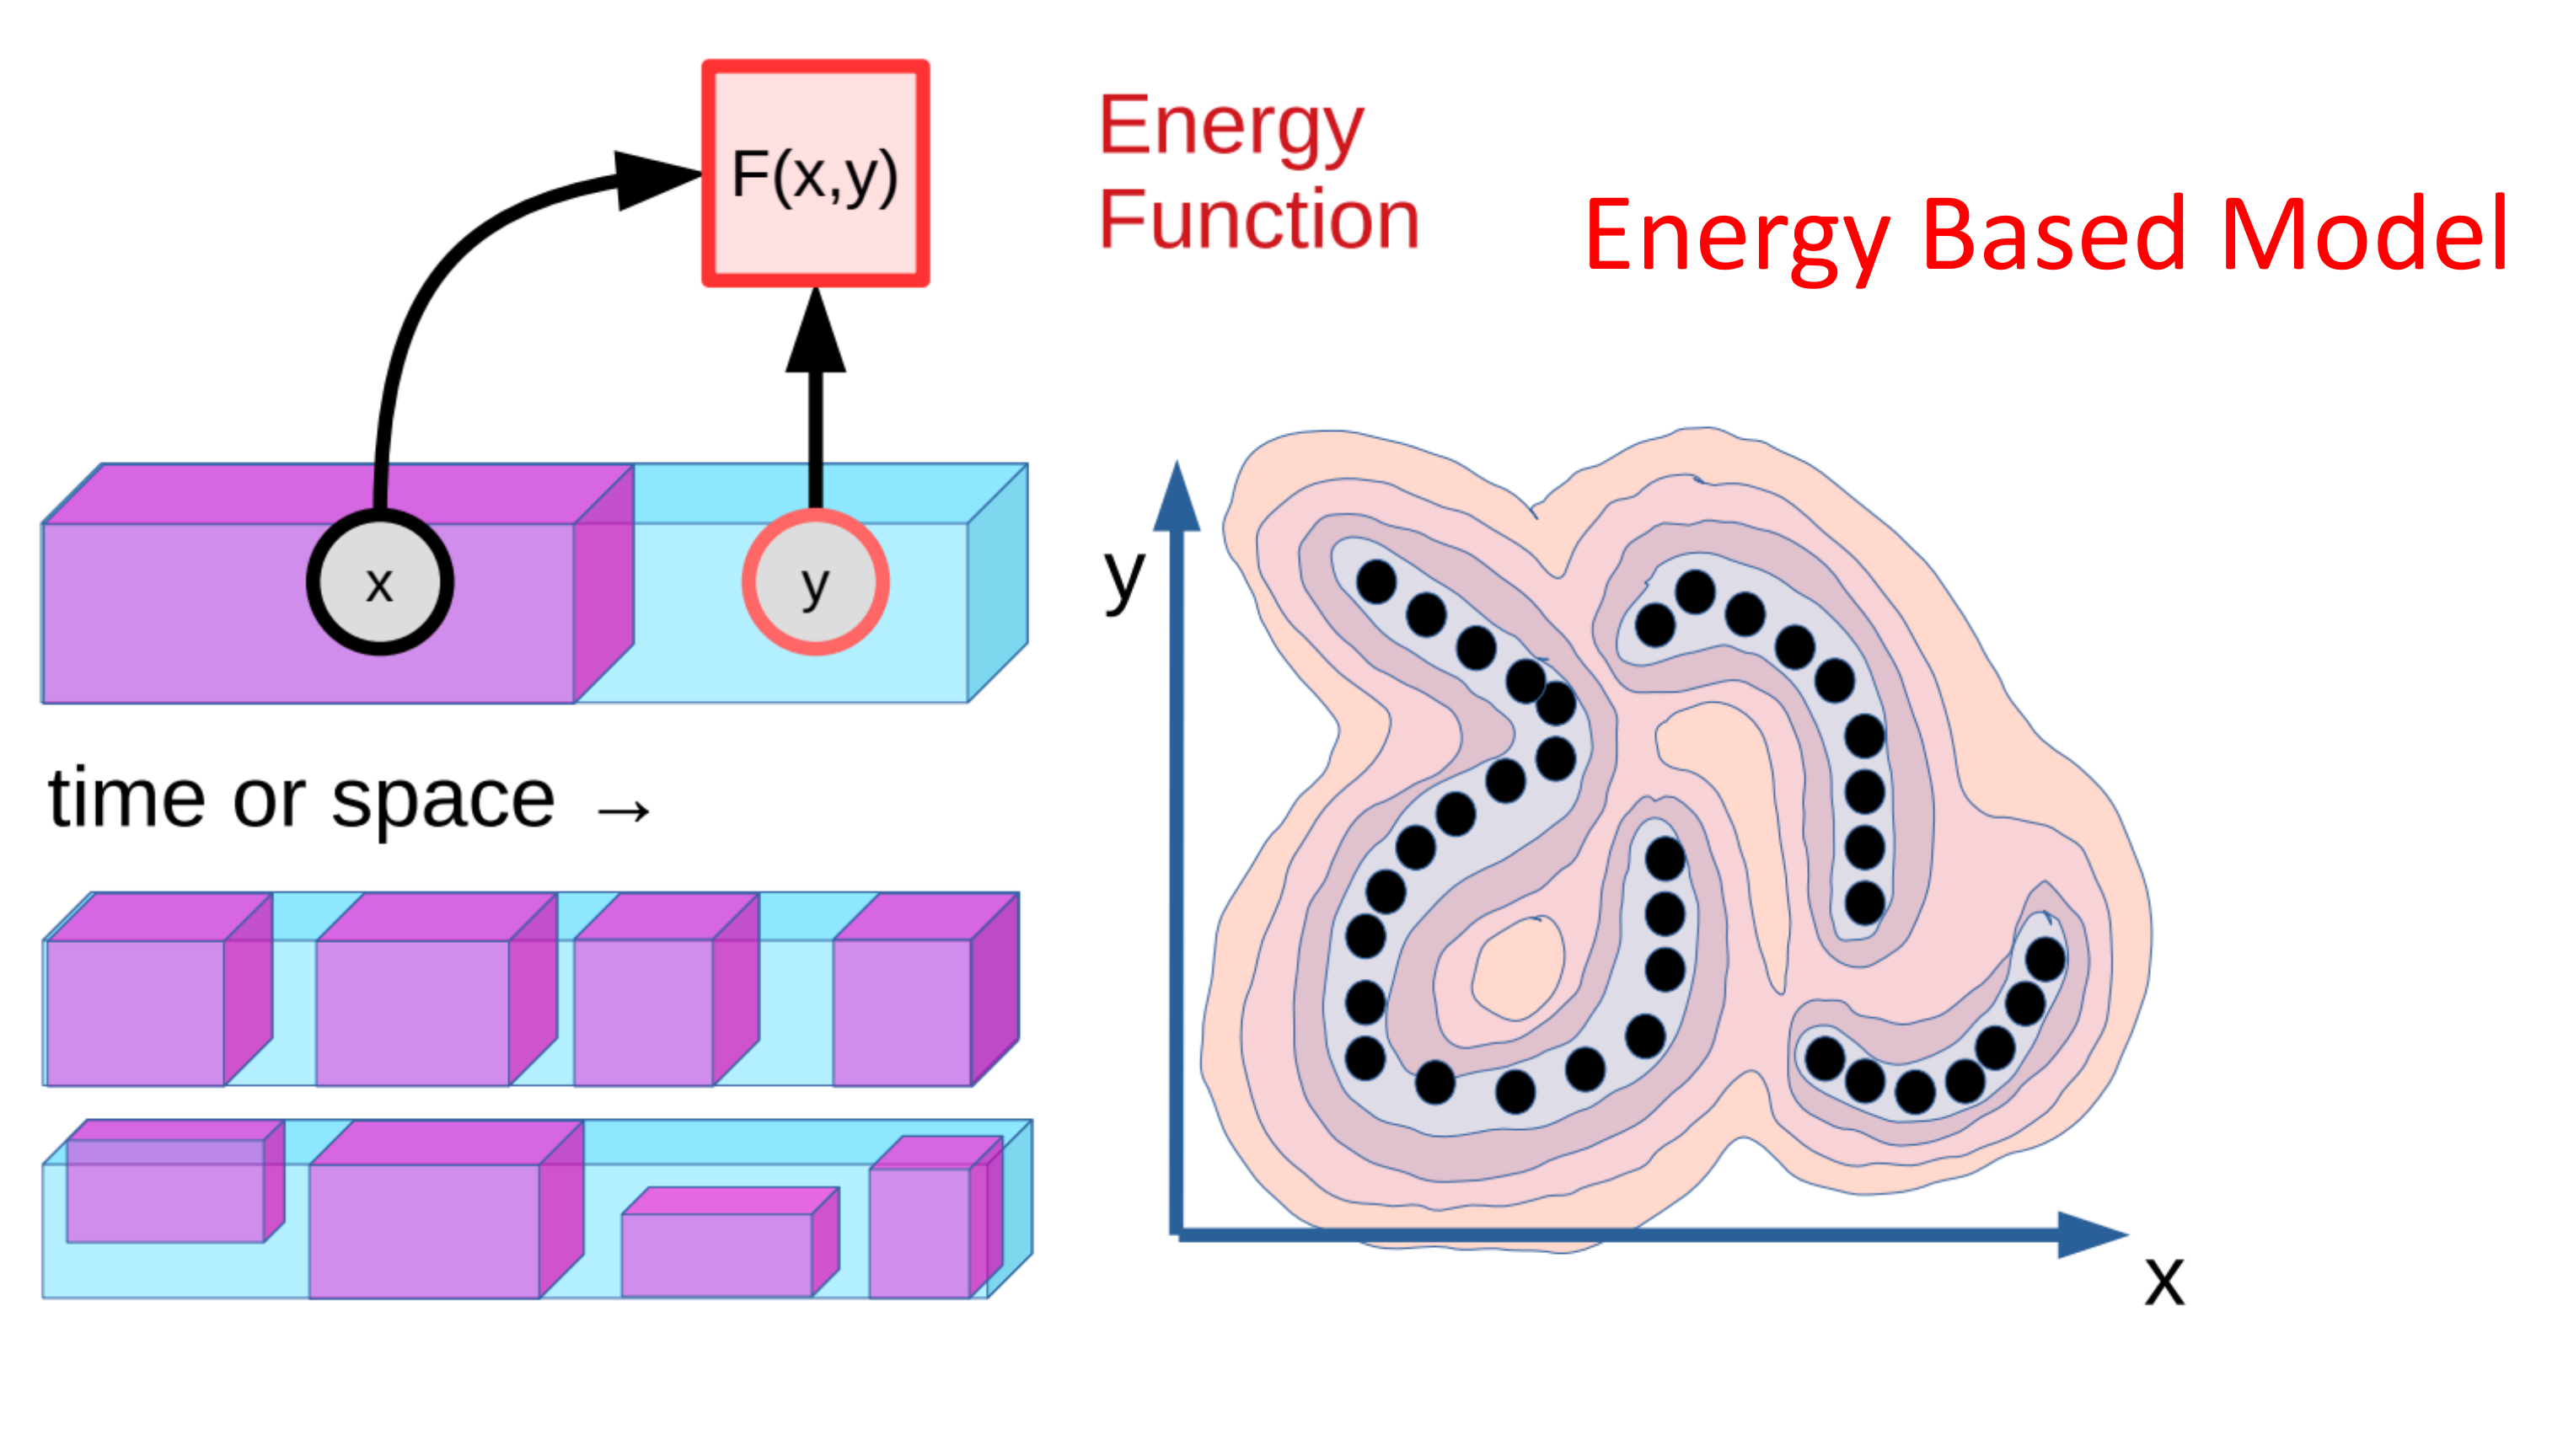
\includegraphics[width=\linewidth,height=0.82\textheight,keepaspectratio]{images/world-models/jepa_cs25_sl06_jepa_lecun_2022_ebm.png}\\[0.08em]
  {\scriptsize Paper: \href{https://openreview.net/forum?id=BZ5a1r-kVsf}{OpenReview}, Y.\ LeCun (2022).}
\end{frame}

\begin{frame}[t]{V-JEPA: video JEPA}
  \centering
  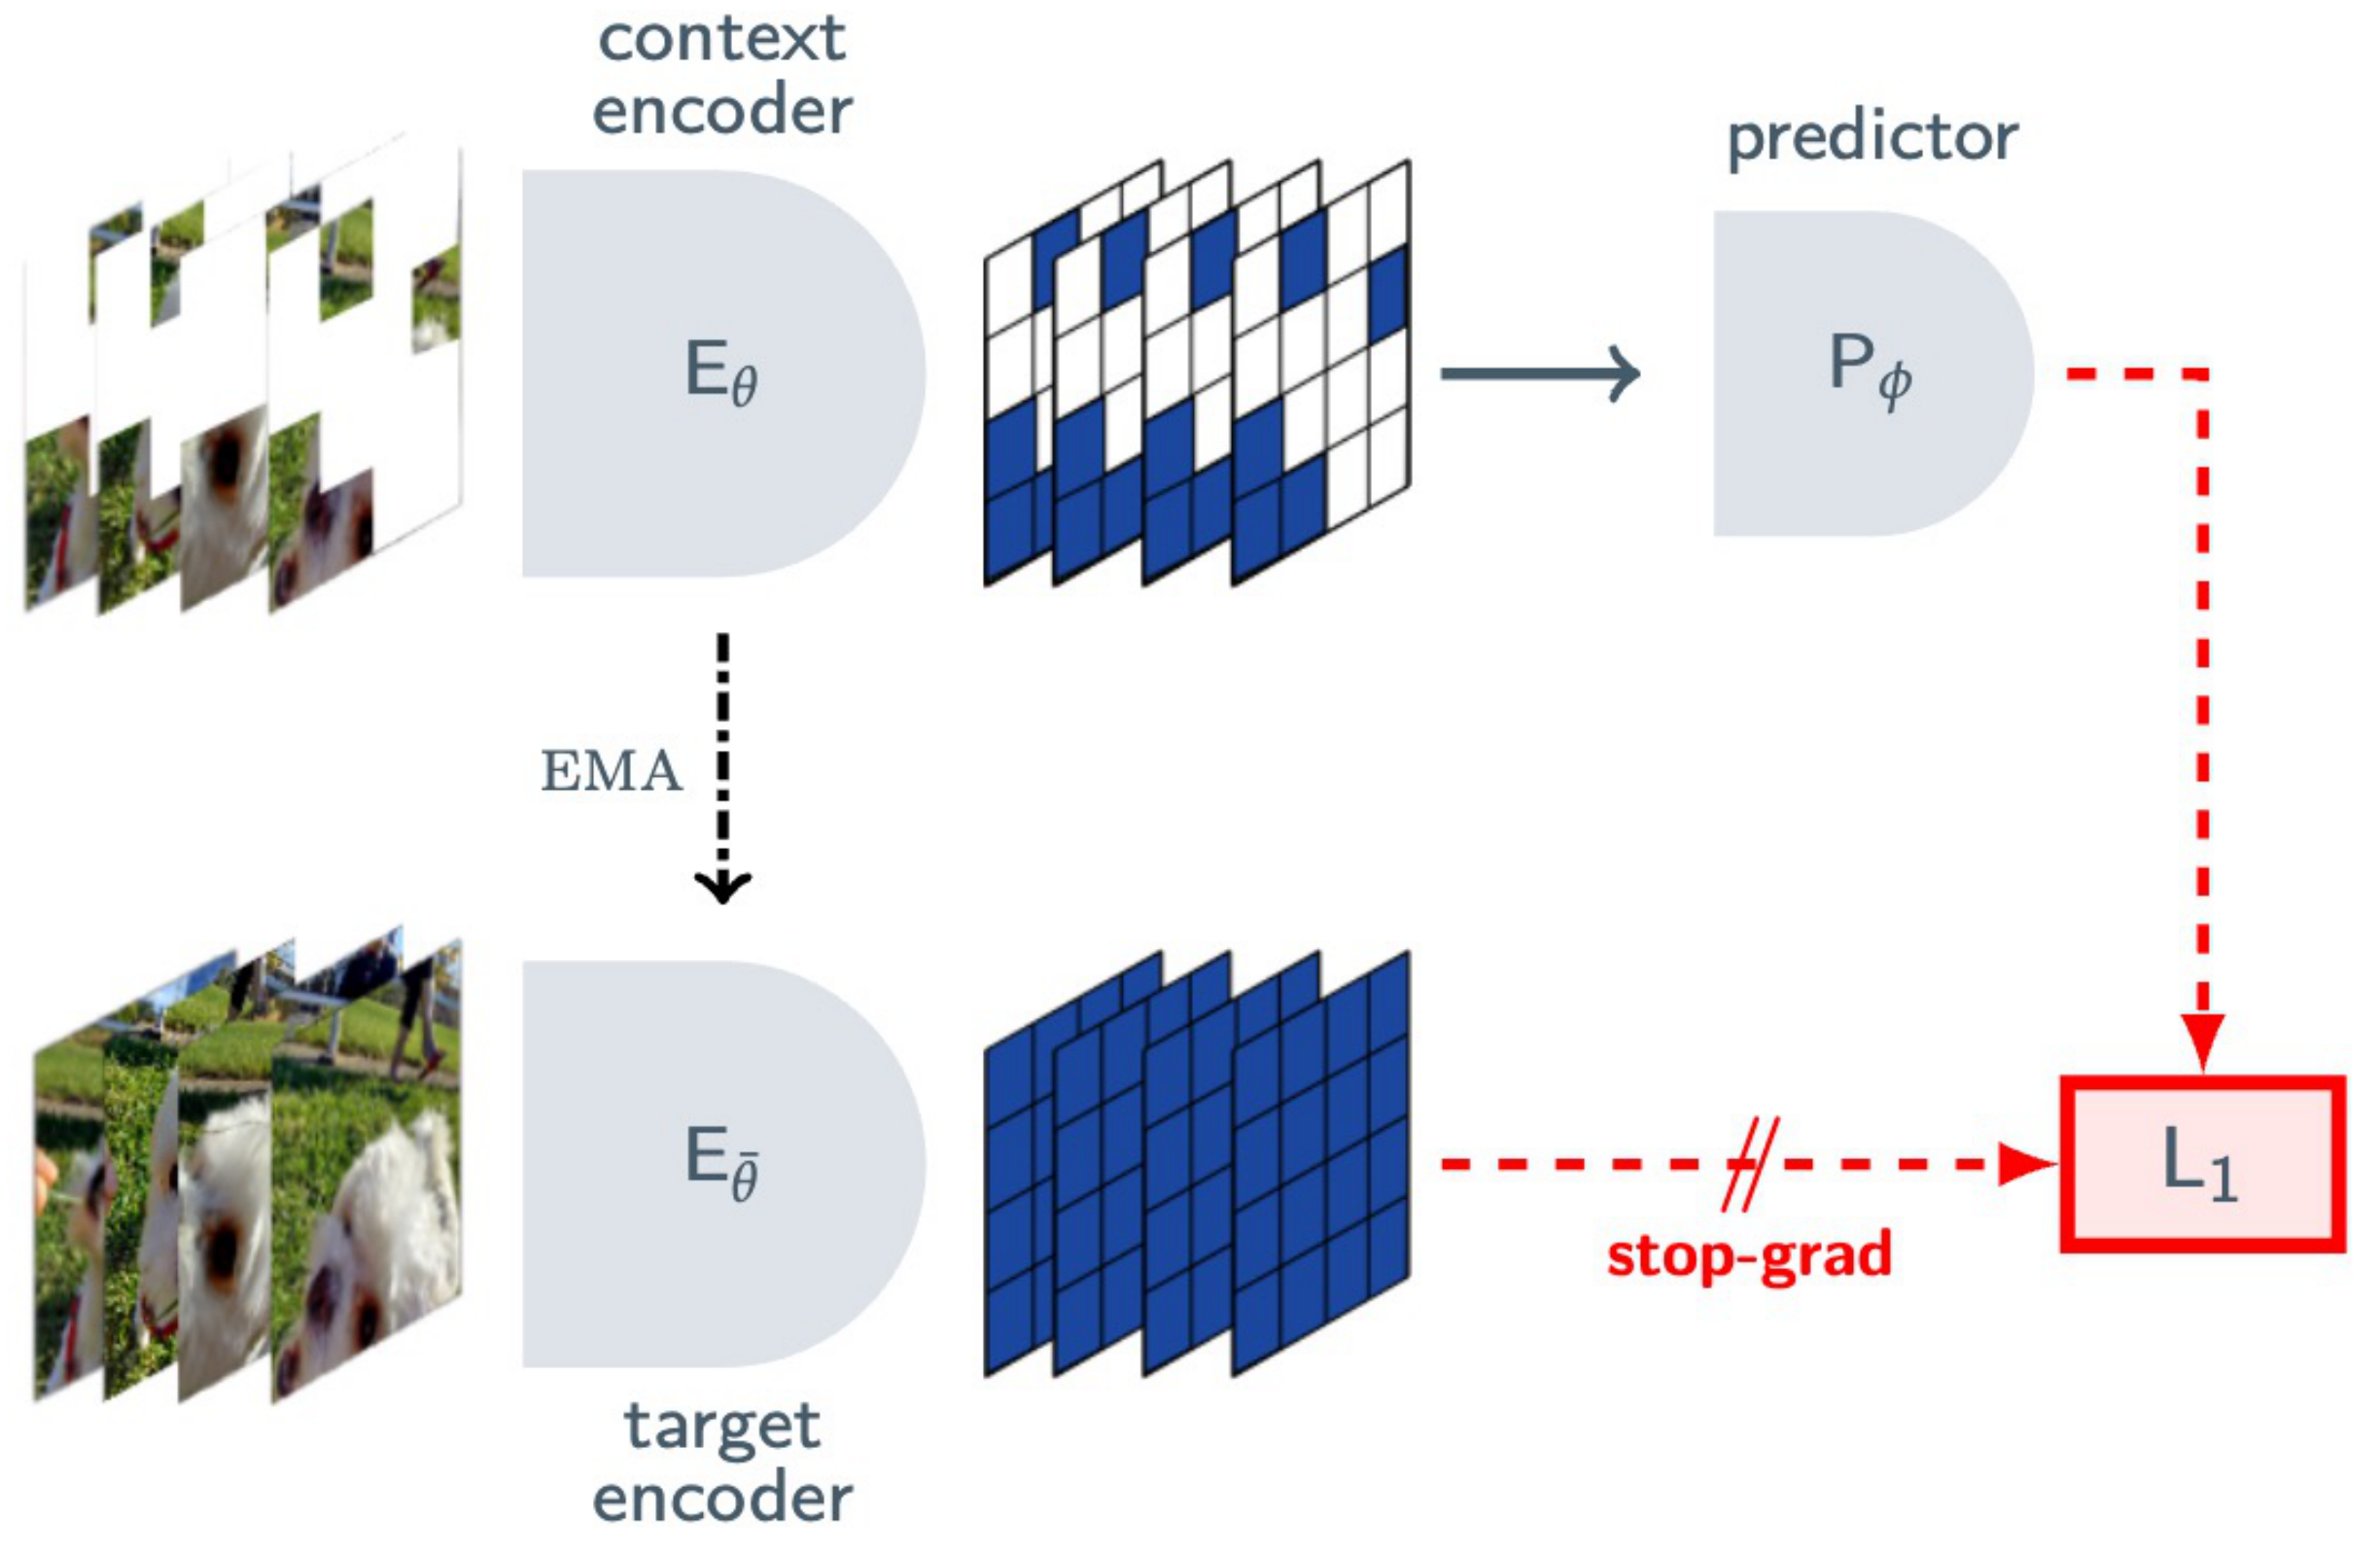
\includegraphics[width=\linewidth,height=0.82\textheight,keepaspectratio]{images/world-models/jepa_cs25_sl07_vjepa_bardes_2024.png}\\[0.08em]
  {\scriptsize Paper: Bardes et al., \href{https://arxiv.org/abs/2404.08471}{arXiv:2404.08471} (V-JEPA).}
\end{frame}

\begin{frame}[t]{V-JEPA\,2: action-conditioned latent prediction}
  \centering
  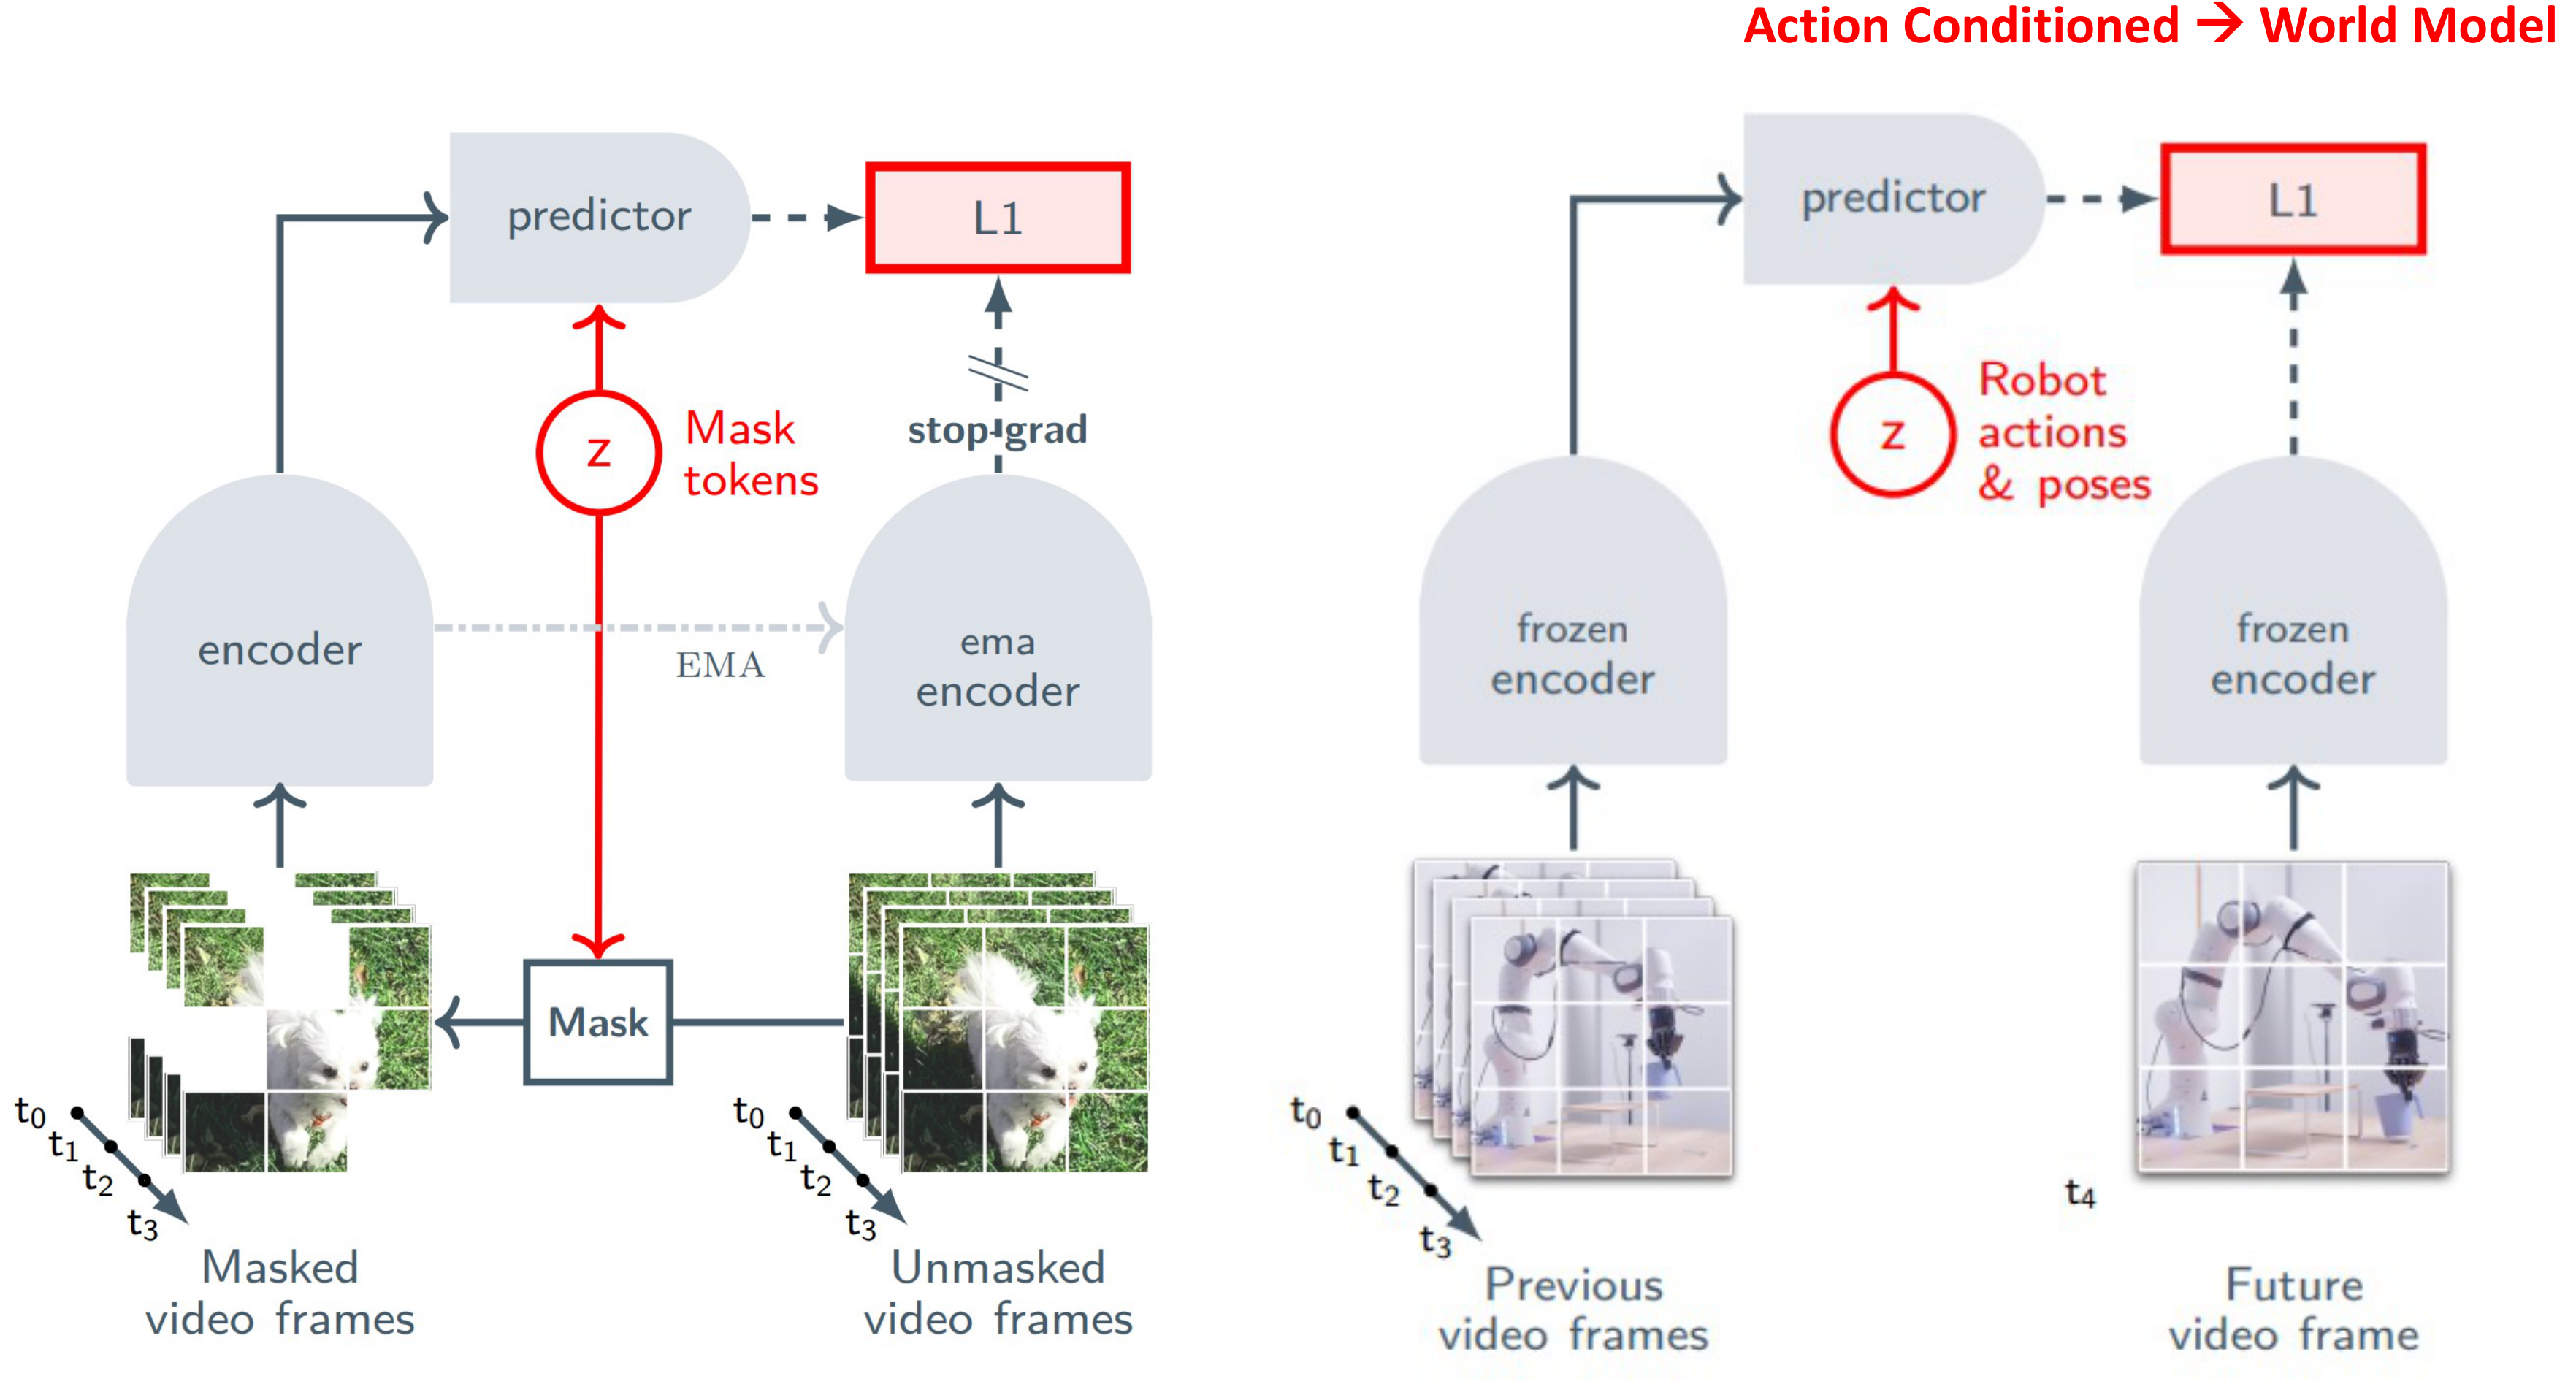
\includegraphics[width=\linewidth,height=0.74\textheight,keepaspectratio]{images/world-models/jepa_cs25_sl08_vjepa2_action_world_model.png}\\[0.04em]
  {\scriptsize Paper: Assran et al., \href{https://arxiv.org/abs/2506.09985}{arXiv:2506.09985} (V-JEPA\,2).}
\end{frame}

\begin{frame}{Generative world models vs.\ JEPA-style prediction}
  \begin{columns}[T,onlytextwidth]
    \column{0.48\textwidth}
    \textbf{Generative (reconstruction) path}\\[0.35em]
    \begin{itemize}\itemsep0.28em
      \item[\textcolor{red}{$\blacktriangleright$}] Learn latents that \textbf{decode} back to pixels (VAE/RSSM).
      \item[\textcolor{red}{$\blacktriangleright$}] Strength: full \textbf{observation model} for planning, denoising, and imagined rollouts with explicit images.
      \item[\textcolor{red}{$\blacktriangleright$}] Cost: optimization can emphasize pixels over semantics.
    \end{itemize}
    \column{0.48\textwidth}
    \textbf{Joint-embedding predictive (JEPA) path}\\[0.35em]
    \begin{itemize}\itemsep0.28em
      \item[\textcolor{red}{$\blacktriangleright$}] Predict \textbf{embeddings} of future or masked regions in \textbf{representation space}.
      \item[\textcolor{red}{$\blacktriangleright$}] Strength: can learn useful \textbf{video/robotics} features without needing to generate every pixel.
      \item[\textcolor{red}{$\blacktriangleright$}] Cost: no pixel rollouts to inspect, and control requires adding an action pathway (V-JEPA 2-AC, LeWM).
    \end{itemize}
  \end{columns}
\end{frame}
